

\documentclass[
  aspectratio=169,
  usenames,
  dvipsnames,
  9pt
]{beamer}
% \usepackage[dvipsnames]{xcolor}
\usepackage[utf8]{inputenc}
\usepackage{amsmath}
\usepackage{setspace} 


\usepackage{subcaption}
\usepackage{mycommands}
\usepackage{nicefrac}
\usepackage{listings}

\usepackage{graphicx,array}
\newcolumntype{C}[1]{>{\centering\let\newline\\\arraybackslash\hspace{0pt}}m{#1}}
\newcolumntype{L}[1]{>{\raggedright\let\newline\\\arraybackslash\hspace{0pt}}m{#1}}
\newcolumntype{R}[1]{>{\raggedleft\let\newline\\\arraybackslash\hspace{0pt}}m{#1}}

\graphicspath{{images/},{diagrams/},{figures/},{../written/images/},{../GraphGym/run/}}

 
 
\newcommand{\twg}[1]{
  \begin{figure}
    \centering
    \includegraphics[width=\textwidth]{#1}
  \end{figure}
}
\newcommand{\twgc}[2]{
 \begin{figure}
    \centering
    \includegraphics[width=\textwidth]{#1}
    \caption{#2}
  \end{figure} 
}

% https://tex.stackexchange.com/questions/102069/make-a-heading-in-beamer
\newcommand\myheading[1]{%
  \par\bigskip
  {\large#1}\par\smallskip}
\newcommand\hd[1]{\myheading{#1}} 

% https://tex.stackexchange.com/a/388900
\setbeamertemplate{itemize item}[circle]

\newcommand{\thirdcol}{\column{0.3\textwidth}}
\newcommand{\twothirdcol}{\column{0.6\textwidth}}
\newcommand{\fourthcol}{\column{0.25\textwidth}}
\newcommand{\halfcol}{\column{0.5\textwidth}}
\newcommand{\seventhcol}{\column{0.7\textwidth}}

\newcommand{\papertitle}[1]{
  \centering
  \textcolor{BlueViolet}{
   #1 
 }
 \\
}

\newcommand{\paperauthors}[1]{
  \footnotesize
  \centering
  \textcolor{gray}{
    \textit{
     #1 
    }
  }
  \\
}

% \captionsetup{font=scriptsize}
\usepackage[labelformat=empty,font={color=gray,scriptsize},justification=centering]{caption}


\setbeamertemplate{navigation symbols}{}%remove navigation symbols

% \usepackage{fontspec}

% \usepackage{tikzsymbols}




% black accent color
\usecolortheme[named=black]{structure}


% less prominent frametitle stuff stuff
\setbeamercolor{frametitle}{fg=black!20}
\setbeamerfont{frametitle}{size=\tiny}


% box styling
% 1- Block title (background and text)
\setbeamercolor{block title example}{fg=white, bg=teal}
\setbeamercolor{block body example}{bg=teal!25}
% smaller text size
\setbeamerfont{block title}{size=\small}
\setbeamerfont{block body}{size=\small}

\newenvironment<>{definitionblock}[1]{%
  \setbeamercolor{block title}{fg=white,bg=purple!45}%
  \setbeamercolor{block body}{bg=purple!10}
  \begin{block}#2{#1}}{\end{block}}




% Information to be included in the title page:
\title{Node Duplication in Disease Maps \\ using Graph Neural Networks}
\author{}
\date{}
\institute{Colloquium}


\begin{document}

\frame{\titlepage}


\begin{frame}
  \frametitle{Introduction / Disease Maps / Examples}
  \begin{columns}
    \halfcol
    \begin{figure}[h]
      \centering
      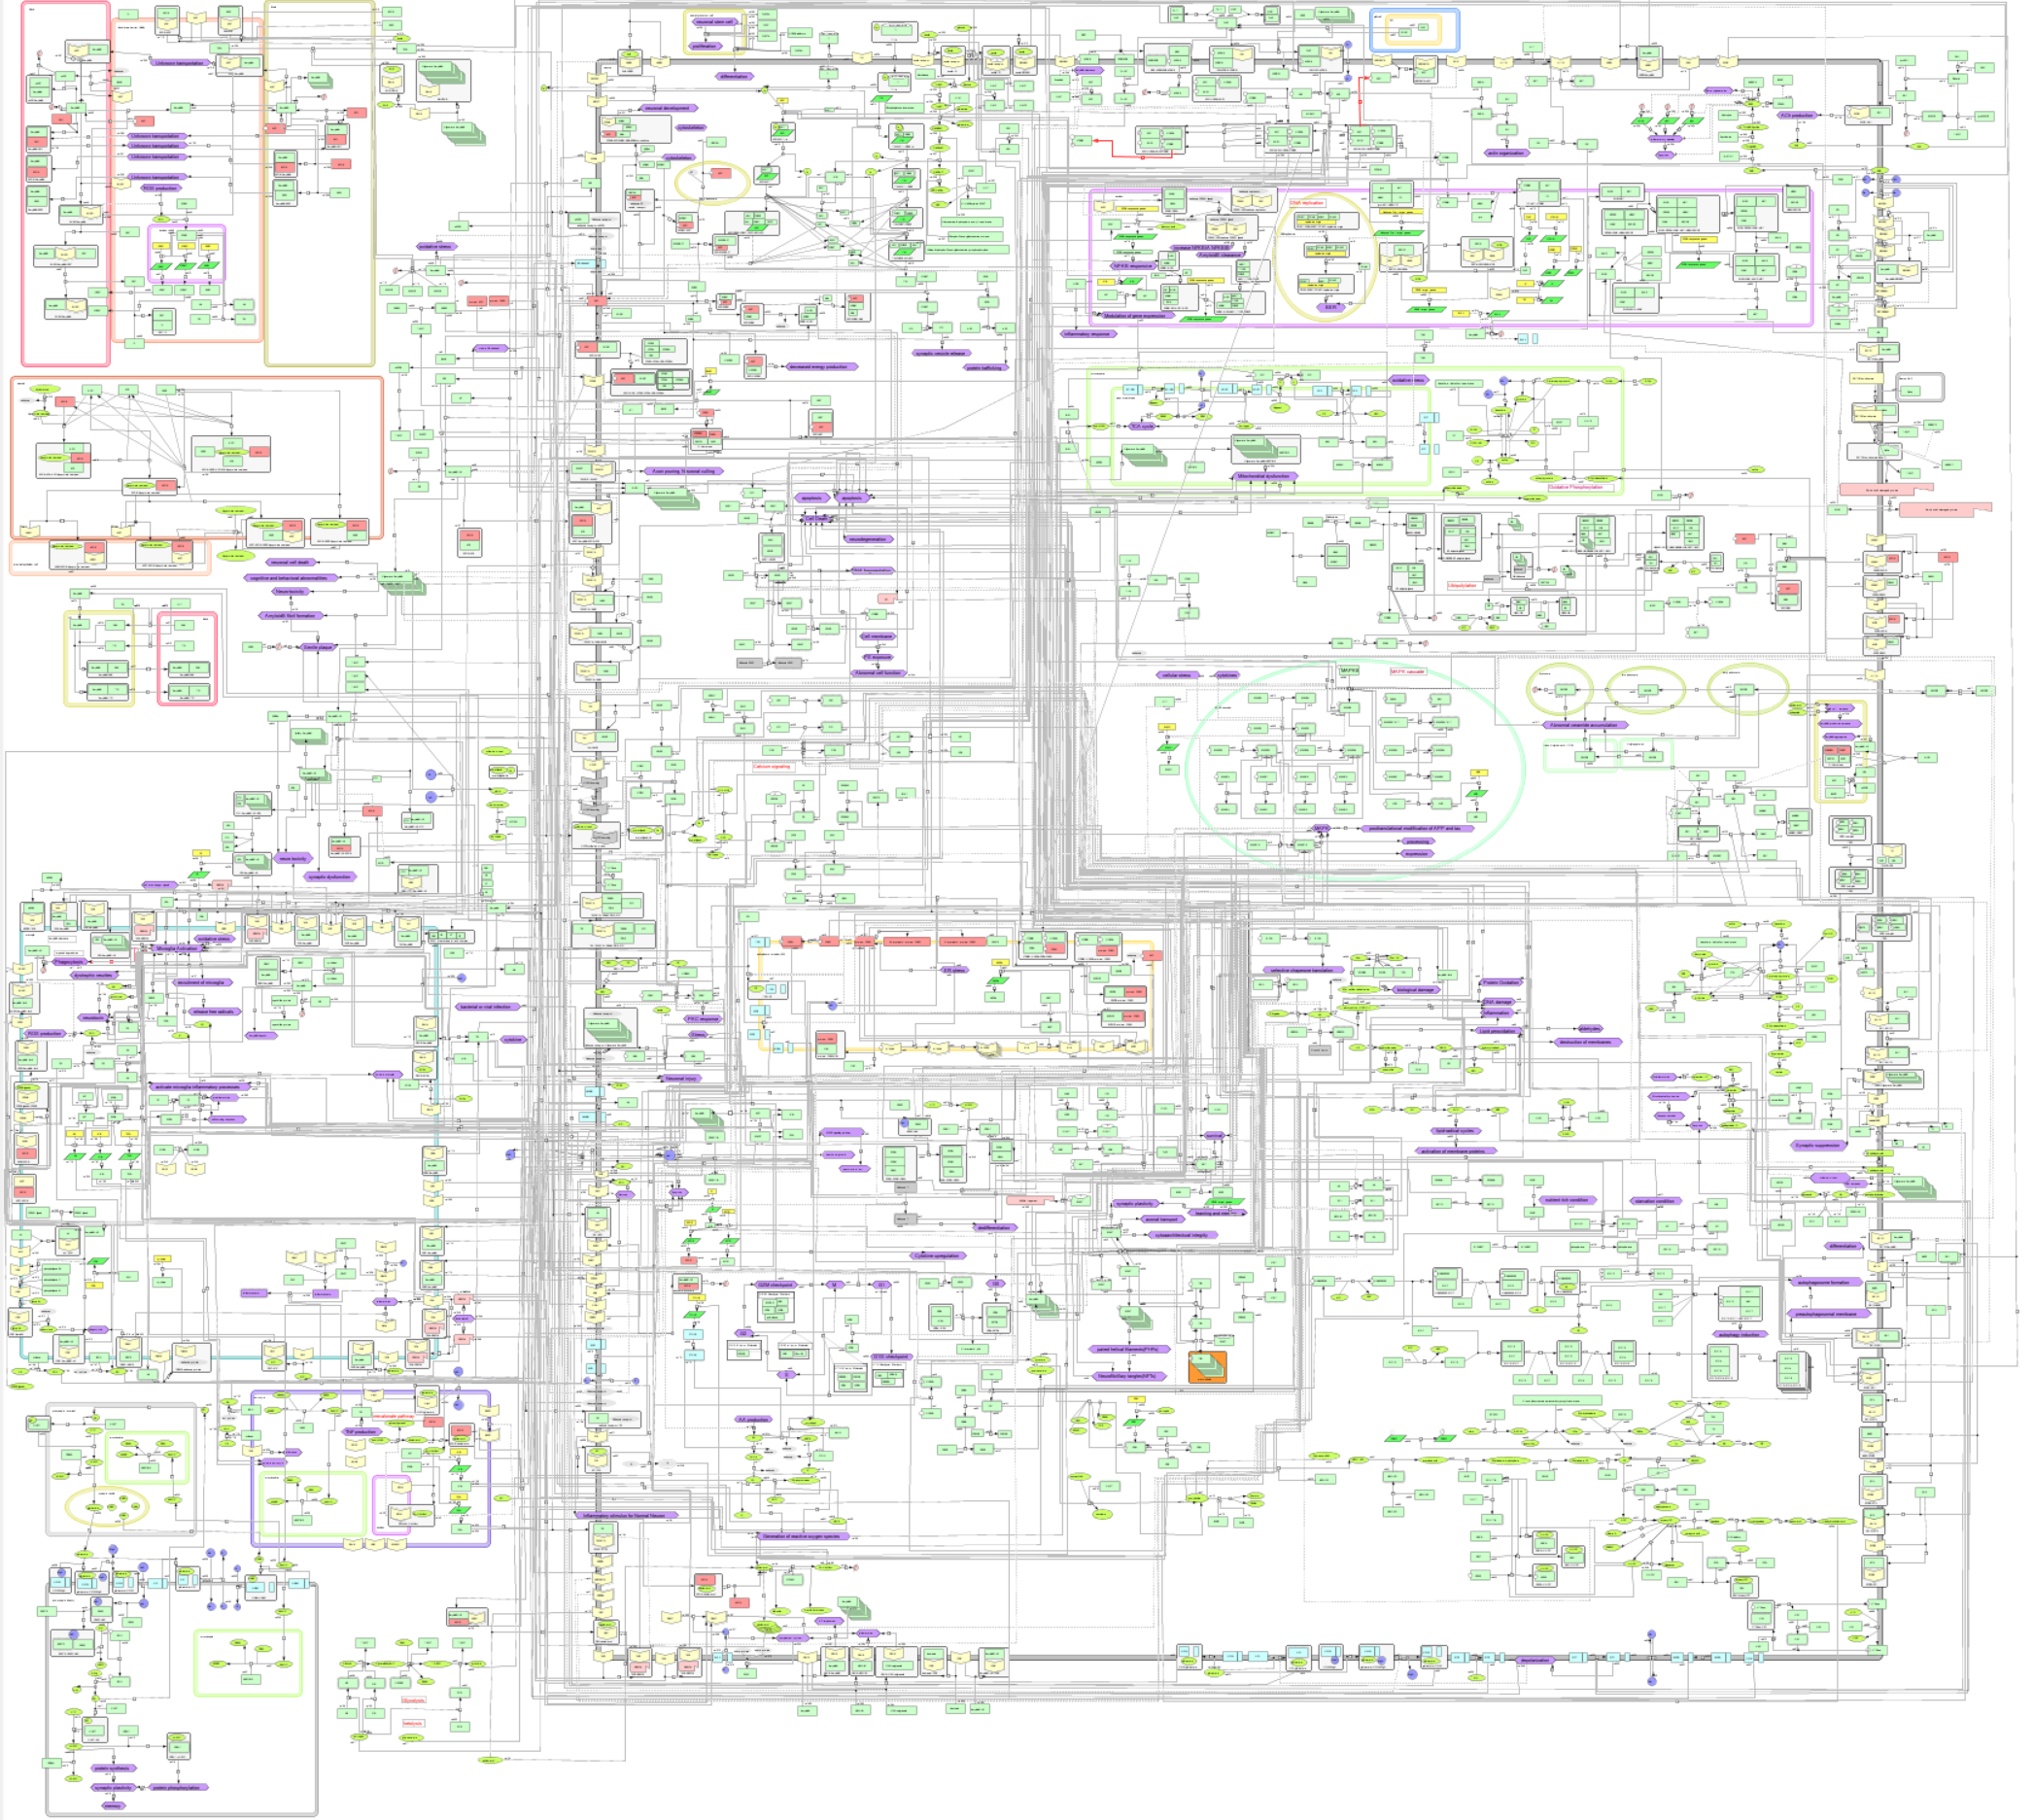
\includegraphics[width=\linewidth]{disease-map-screenshots/alzpathway/201.png}
    \end{figure}
    \halfcol
    \begin{itemize}
    \item Can always make layout task easier by duplicating nodes with degree
      $\geq 2$
      \item But which nodes can be duplicated s.t. network information remains faithful?
    \end{itemize}
  \end{columns}
\end{frame}

\begin{frame}
  \frametitle{TODO}

  \begin{tabular}{C{2.8cm}  L{8.5cm}}
    % TODO add some words about how this is likely due to the interconnecte
    % nature of biological systems?
    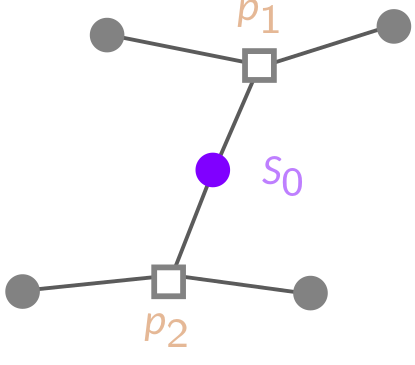
\includegraphics[width=0.7\linewidth]{true-false-connectivity-connected.png} &
    Single species alias may be connecting multiple processes \\[3em]
    % 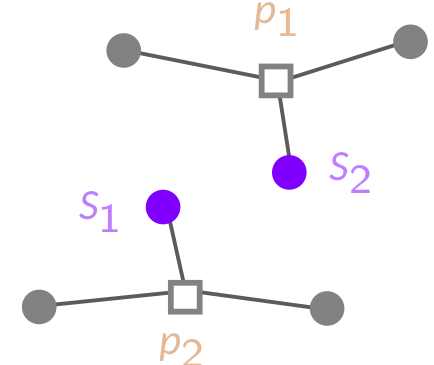
\includegraphics[width=0.7\linewidth]{true-false-connectivity-duplicated.png} & Path $(p_1, S_0, p_2)$ is not meaningful $\leadsto$ \ild{duplicate} $S_0$ \\[4em]
    % 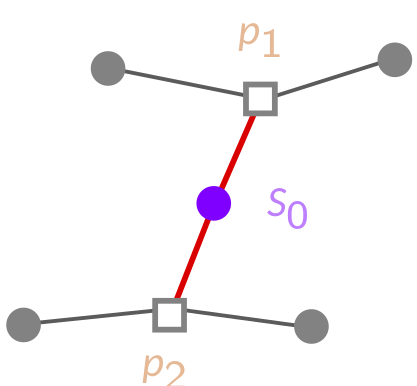
\includegraphics[width=0.7\linewidth]{true-false-connectivity-key-connector} & Path is meaningful $\leadsto$ $S_0$ must not be duplicated
  \end{tabular}

  \begin{definitionblock}{}
    \vspace{0.5em}
    \begin{columns}
      \column{8.5cm}
      Path $(p_1, S_0, p_2)$ is semantically meaningful
      (\ild{true connectivity})
      \\[1em]
      {\footnotesize
        $\leadsto$ $S_0$ must not be duplicated
      }
      \column{2.8cm}
      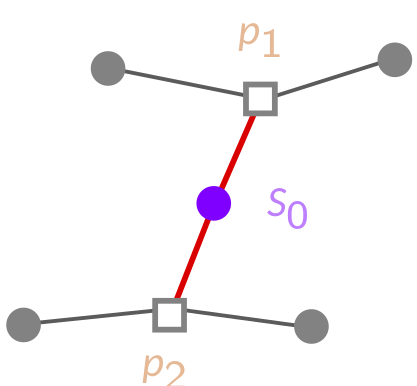
\includegraphics[width=0.7\linewidth]{true-false-connectivity-key-connector.png}
    \end{columns}
    \vspace{0.5em}
  \end{definitionblock}


  \begin{definitionblock}{}
    \vspace{0.5em}
    \begin{columns}
      \column{8.5cm}
      Path $(p_1, S_0, p_2)$ is not meaningful
      (implies \ild{false connectivity})
      \\[1em]
      {\footnotesize
        There should be no paths implying false connectivity \\ $\leadsto$ $S_0$ should be \ild{duplicated}
      }
      % TODO here we sort of pre-empt criteria for duplication
      \column{2.8cm}
      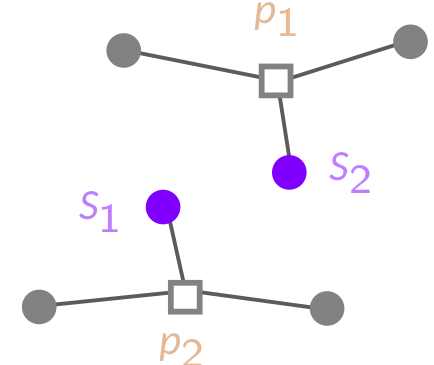
\includegraphics[width=0.7\linewidth]{true-false-connectivity-duplicated.png}
    \end{columns}
    \vspace{0.5em}
  \end{definitionblock}
  {\footnotesize
    e.g. due to unrelated roles of $S_0$ in $p_1$, $p_2$, not stoichiometrically
    linked, unimportant byproduct
  }
  
\end{frame}  


\begin{frame}
  \frametitle{TODO}
  \begin{exampleblock}{Objective 1}
    Assess whether a given species alias implies false connectivity (and should
    thus be duplicated)
  \end{exampleblock}
  here: depends on context etc.?
  \begin{exampleblock}{Objective 2}
    Determine number of duplicates and attachment of edges
  \end{exampleblock}
\end{frame}


\begin{frame}
  \frametitle{Related Work}
  Some previous approaches would rely on \textbf{node centrality scores}

  high centrality $\leadsto$ heterogeneous neighbourhood $\leadsto$ false
  connectivity

  \begin{itemize}
  \item node degree
   \cite{ma_ReconstructionMetabolicNetworks_2003, schuster_exploring_2002} 
 \item eigenvector centrality
  \cite{manipur_clustering_2020} 
  \item communities (modularity)
    \begin{itemize}
    \item contribution to modularity if node removed 
      \cite{huss_CurrencyCommodityMetabolites_2007}
    \item based on intra- \& inter-community degrees
     \cite{guimera_FunctionalCartographyComplex_2005} 
    \end{itemize}
    \item communities (semantic)
      \begin{itemize}
      \item cellular compartment 
        \cite{manipur_clustering_2020}
      \item pathway annotation
        \cite{rohrschneider_NovelGridBasedVisualization_2010,joshi-tope_ReactomeKnowledgebaseBiological_2005,lambert_PathwayPreservingRepresentation_2011}
      \end{itemize}
  \end{itemize}
\end{frame}


\begin{frame}
  \frametitle{TODO}
  (motivation for ML approach)
\end{frame}


\begin{frame}
  \frametitle{Problem Definition / Overview}
  \begin{exampleblock}{Objective}
      Given expert decisions, train an ML model to predict node duplication.
  \end{exampleblock}

  \begin{figure}[h]
    \centering
    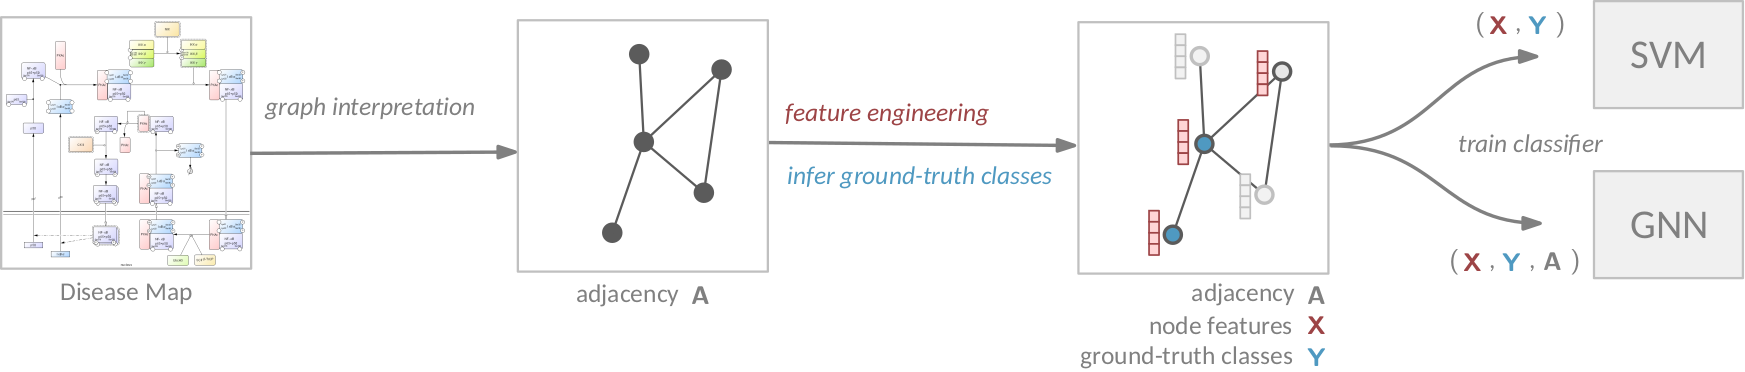
\includegraphics[width=\textwidth]{pipeline.png}
  \end{figure}

\end{frame}

 

\begin{frame}
  % TODO schematic for TPR, TPR
  \frametitle{Problem Definition / Evaluation of Classifiers / Precision \& Recall}
  \begin{itemize}
  \item To compare classifiers, we need an \textbf{unbiased performance measure}
  \end{itemize}
  \begin{itemize}
  \item Classifiers yield a \ild{confidence score} in $[0,1]$ for a given example
  \item Obtain concrete classification by setting a \ild{decision threshold}
  \end{itemize}
  % not analog. to precision-recall curve since recall is sensitive to
  % class skew  -- does not make sense to introduce Precision and Recall then,
  % simply stick to TPR, FPR
  \begin{itemize}
    \item \ild{True Positive Rate} (\TPR{}): $\nicefrac{\text{\# true
          positives}}{\text{\# actually positive}}$
      \item \ild{False Positive Rate} (\FPR{}): $\nicefrac{\text{\# false
            positives}}{\text{\# actually negative}}$
  % \item \ild{Precision}: $\nicefrac{\text{\# true positives}}{\text{\# predicted
  %       positive}} = 1 - \FPR{}$
  % \item \ild{Recall} (or True Positive Rate): $\nicefrac{\text{\# true
  %       positives}}{\text{\# actually positive}}$
  \end{itemize}
  \begin{itemize}
  \item Usually a tradeoff, choice depends on use-case
    \begin{itemize}
      \footnotesize
      \item Accept only few high-confidence predictions $\rightarrow$ low
        \FPR{}, but also low \TPR{} (Recall)
      \item Lower decision threshold $\rightarrow$ increase \TPR{} at cost of
        increased \FPR{}
    % \item Accept only high-confidence predictions $\rightarrow$ high precision, low recall
    % \item Lower decision threshold $\rightarrow$ increase recall at cost of precision
    \end{itemize}
  \end{itemize}
\end{frame}

\begin{frame}
  \frametitle{Problem Definition / Evaluation of Classifiers / ROC Curve}
  \begin{columns}
    \halfcol
    \begin{figure}[h]
      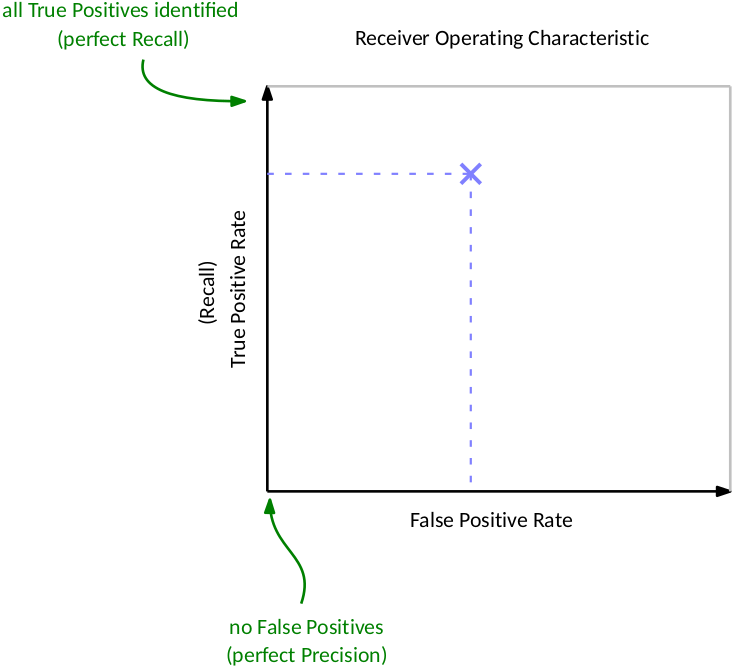
\includegraphics[width=7cm]{roc-intro.png}
    \end{figure}
    \halfcol
    \begin{itemize}
    \item Concrete choice of threshold yields binary classification and \TPR{}, \FPR{}
    \end{itemize}
  \end{columns}
\end{frame}

\begin{frame}
  \frametitle{Problem Definition / Evaluation of Classifiers / ROC Curve}
  \begin{columns}
    \halfcol
    \begin{figure}[h]
      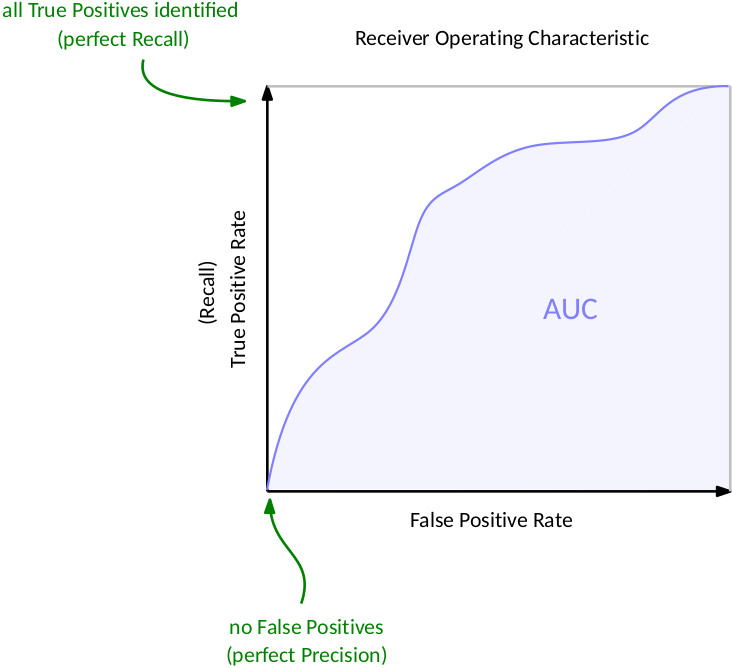
\includegraphics[width=7cm]{roc-intro-line.png}
      \caption{Plot \TPR{} and \FPR{} as function of decision threshold}
    \end{figure}
    \halfcol %
    \begin{itemize}
    \item Plot \TPR{}, \FPR{} as function of decision threshold $\leadsto$ \ild{ROC
        curve}
    \item Useful properties:
      \begin{itemize}
      \item Show overall behaviour with respect to variable threshold
      \item Insensitive to class distribution
        % If the proportion of positive to negative instances changes in a test set,
        % the ROC curves will not change.
      \item Insensitive to error costs
      \end{itemize}
    \end{itemize}
  \end{columns}
\end{frame}





\begin{frame}
  \frametitle{Block Example}
  \begin{figure}[h]
    \centering
    \begin{subfigure}[h]{0.49\linewidth}
      \centering
      \includegraphics[width=0.9\linewidth]{svm-repro-repeats/results/comparison/roc.png}
      \caption{(\ADMap{} $\rightarrow$ \PDMap)}
    \end{subfigure}
    \begin{subfigure}[h]{0.49\linewidth}
      \centering
      \includegraphics[width=0.9\linewidth]{svm-repro-reconmapolder-repeats/results/comparison/roc.png}
      \caption{(\ADMap{} $\rightarrow$ \ReconMap)}
    \end{subfigure}
    \caption{foo}
    \label{fig:svm-repro-results}
  \end{figure}
  \vspace{-1em}
  \begin{exampleblock}{}
    \begin{itemize}
    \item foo bar baz flubble qox cazinga
    \item flofola kinorrat ewusa a 
    \end{itemize}
  \end{exampleblock}
\end{frame}


% \begin{frame}
%   Thanks for listening 
% 	\Laughey[1.4] \\
% \end{frame}


\section{References}

\begin{frame}[allowframebreaks]
	% \nocite{*}
  \footnotesize
	% \bibliographystyle{unsrt} % sort by appereance in text
	\bibliography{../written/BA.bib}
\end{frame}

\end{document}

